\section{Experimental Results}
\label{section:exp}

\subsection{Experimental Setup}
\label{section:exp:setup}

All RL agents share a single DQN configuration; the two variants differ only in whether the learning-curve derivative features (Section~\ref{section:algorithm}) are appended to the state. The Q-network is a single-layer LSTM with hidden size 64: the 16-dimensional, $L_2$-normalized dataset descriptor is projected by two linear layers to initialize the recurrent hidden and cell states $(h_0, c_0)$, and the final hidden state is mapped to per-action Q-values by a two-layer MLP head ($64 \rightarrow 64 \rightarrow |\mathcal{A}|$ with ReLU). At each step the state is a zero-padded sequence of history rows, where each row concatenates the encoded configuration, the scalar improvement reward, the five derivative statistics (\texttt{LC-DQN} only), and the static descriptor. The action space $\mathcal{A}$ is the benchmark's precomputed configuration grid (sampled without replacement within an episode), and the reward is the validation-loss improvement $r_t = \max(0,\, f_{t-1} - f_t)$. Training follows standard DQN with a hard-updated target network, Bellman target $r + \gamma \max_{a'} Q_{\text{target}}(s', a')(1 - \text{done})$, and an MSE temporal-difference loss optimized with Adam. The shared hyperparameters are listed in Table~\ref{tab:dqn_hparams}.

\begin{table}[htbp]
\centering
\caption{DQN agent and meta-training hyperparameters. $E$ denotes the number of meta-training episodes and $T$ the per-episode training budget (HPO rollout length).}
\label{tab:dqn_hparams}
\begin{tabular}{ll}
\toprule
Hyperparameter & Value \\
\midrule
Q-network & 1-layer LSTM (hidden $64$) + MLP head ($64\!\rightarrow\!64\!\rightarrow\!|\mathcal{A}|$) \\
Optimizer & Adam \\
Learning rate & $1 \times 10^{-3}$ \\
Discount factor $\gamma$ & $0.99$ \\
Replay buffer size & $\max(10^4,\; E \cdot T)$ \\
Batch size & $4$ \\
Learning starts & $2$ transitions \\
Target-network update & hard copy every $4$ steps \\
Exploration $\varepsilon$ (meta-training) & linear $1.0 \rightarrow 0.05$ over $E$ episodes \\
Exploration $\varepsilon$ (frozen evaluation) & $0.01$ \\
Meta-training episodes $E$ & $150$ \\
Training budget $T$ & LCBench: $\{20, 50, 100, 150\}$; \quad Kaggle: $20$ \\
Evaluation budget & $20$ \\
\bottomrule
\end{tabular}
\end{table}

The two benchmarks differ only in their task collections and evaluation protocol. On \textbf{LCBench} we meta-train across all 35 OpenML datasets (shared 7-dimensional search space, up to 2{,}000 logged configurations per dataset with 50-epoch curves) using a single seed, and sweep the training budget $T \in \{20, 50, 100, 150\}$ while holding the per-task evaluation budget fixed at 20 (Figure~\ref{fig:hpo_results}). On the \textbf{Kaggle Playground Series} we use 15 heterogeneous tasks (256 cached configurations per task with 25-epoch curves), 5 random seeds, and a single training budget $T = 20$. Across both benchmarks the non-meta baselines (Random Search, Bayesian Optimization) are reinitialized per target task under the same evaluation budget, and the meta-trained policies are frozen after meta-training before evaluation.

\subsection{Evaluation of Baseline Methods}
\label{section:exp:baseline}

Based on the experimental results evaluating validation scores against evaluation budgets, the following technical observations are made regarding the performance of the optimization algorithms:

\begin{figure}[htbp]
    \centering
    \begin{subfigure}[b]{0.48\textwidth}
        \centering
        % Insert the 20 budget image here
        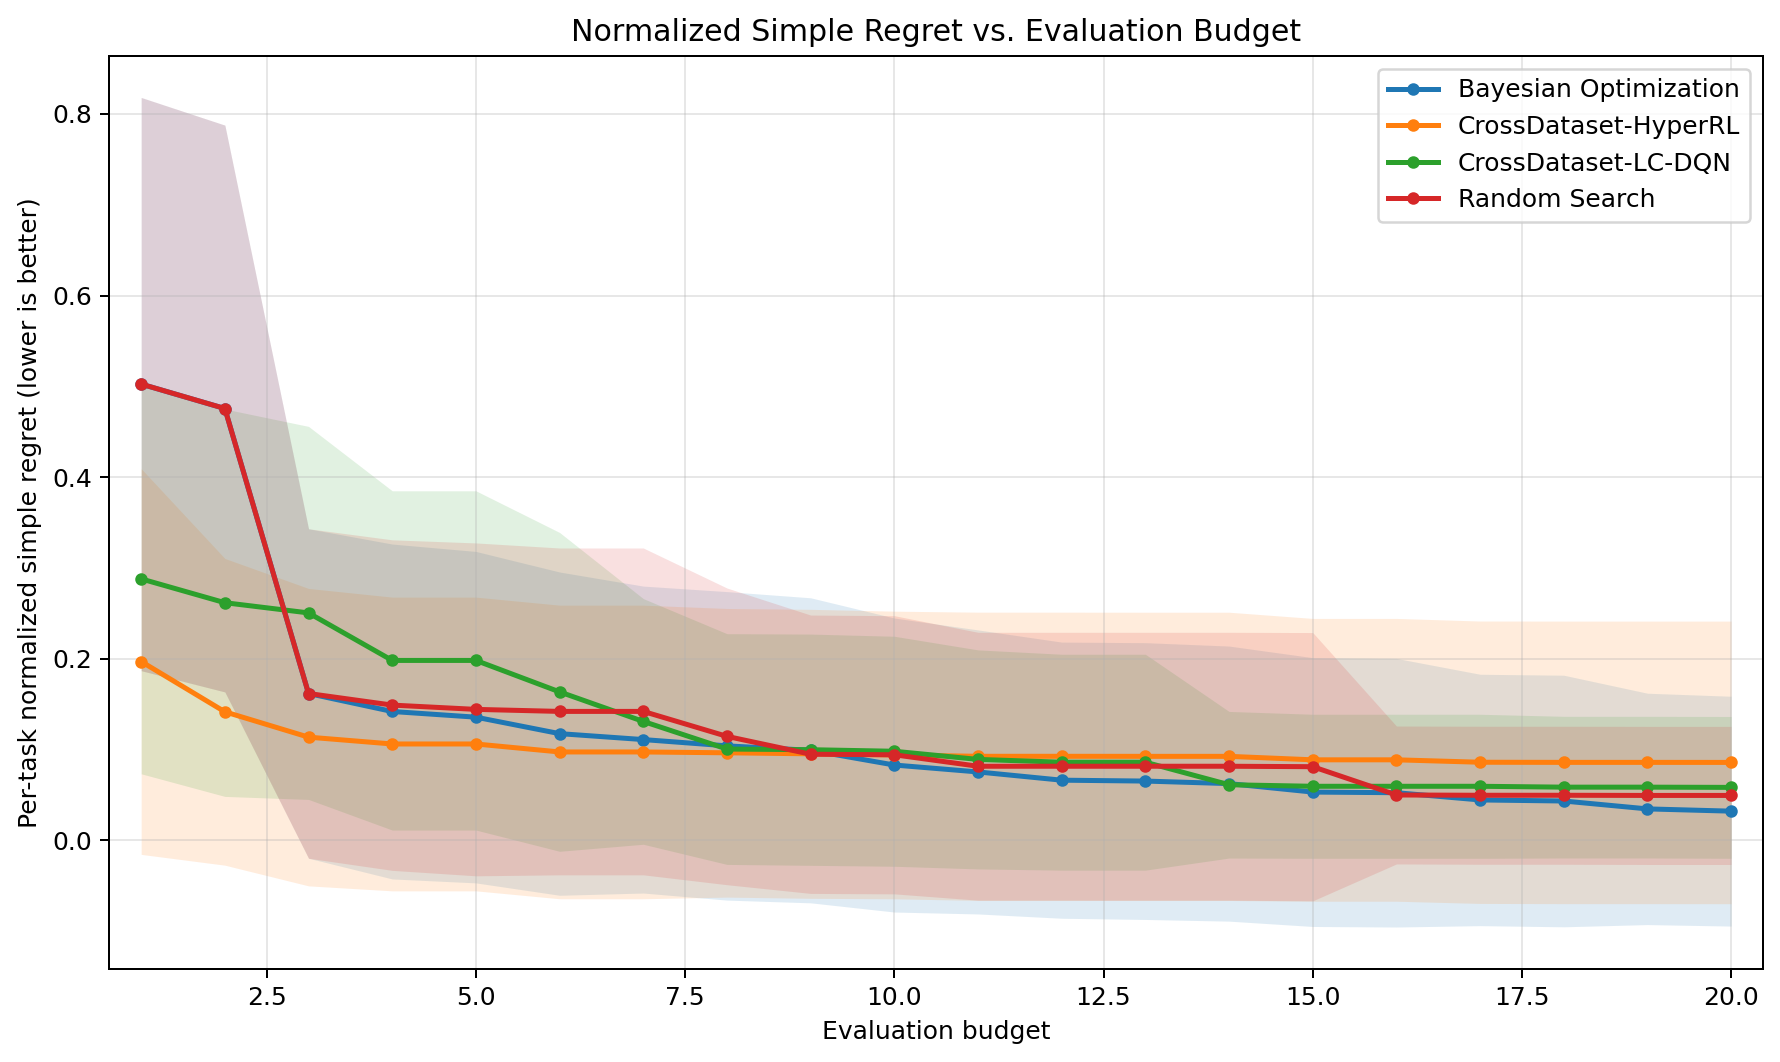
\includegraphics[width=\textwidth]{images/20_budget.png}
        \caption{Training Budget: 20}
        \label{fig:budget_20}
    \end{subfigure}
    \hfill
    \begin{subfigure}[b]{0.48\textwidth}
        \centering
        % Insert the 50 budget image here
        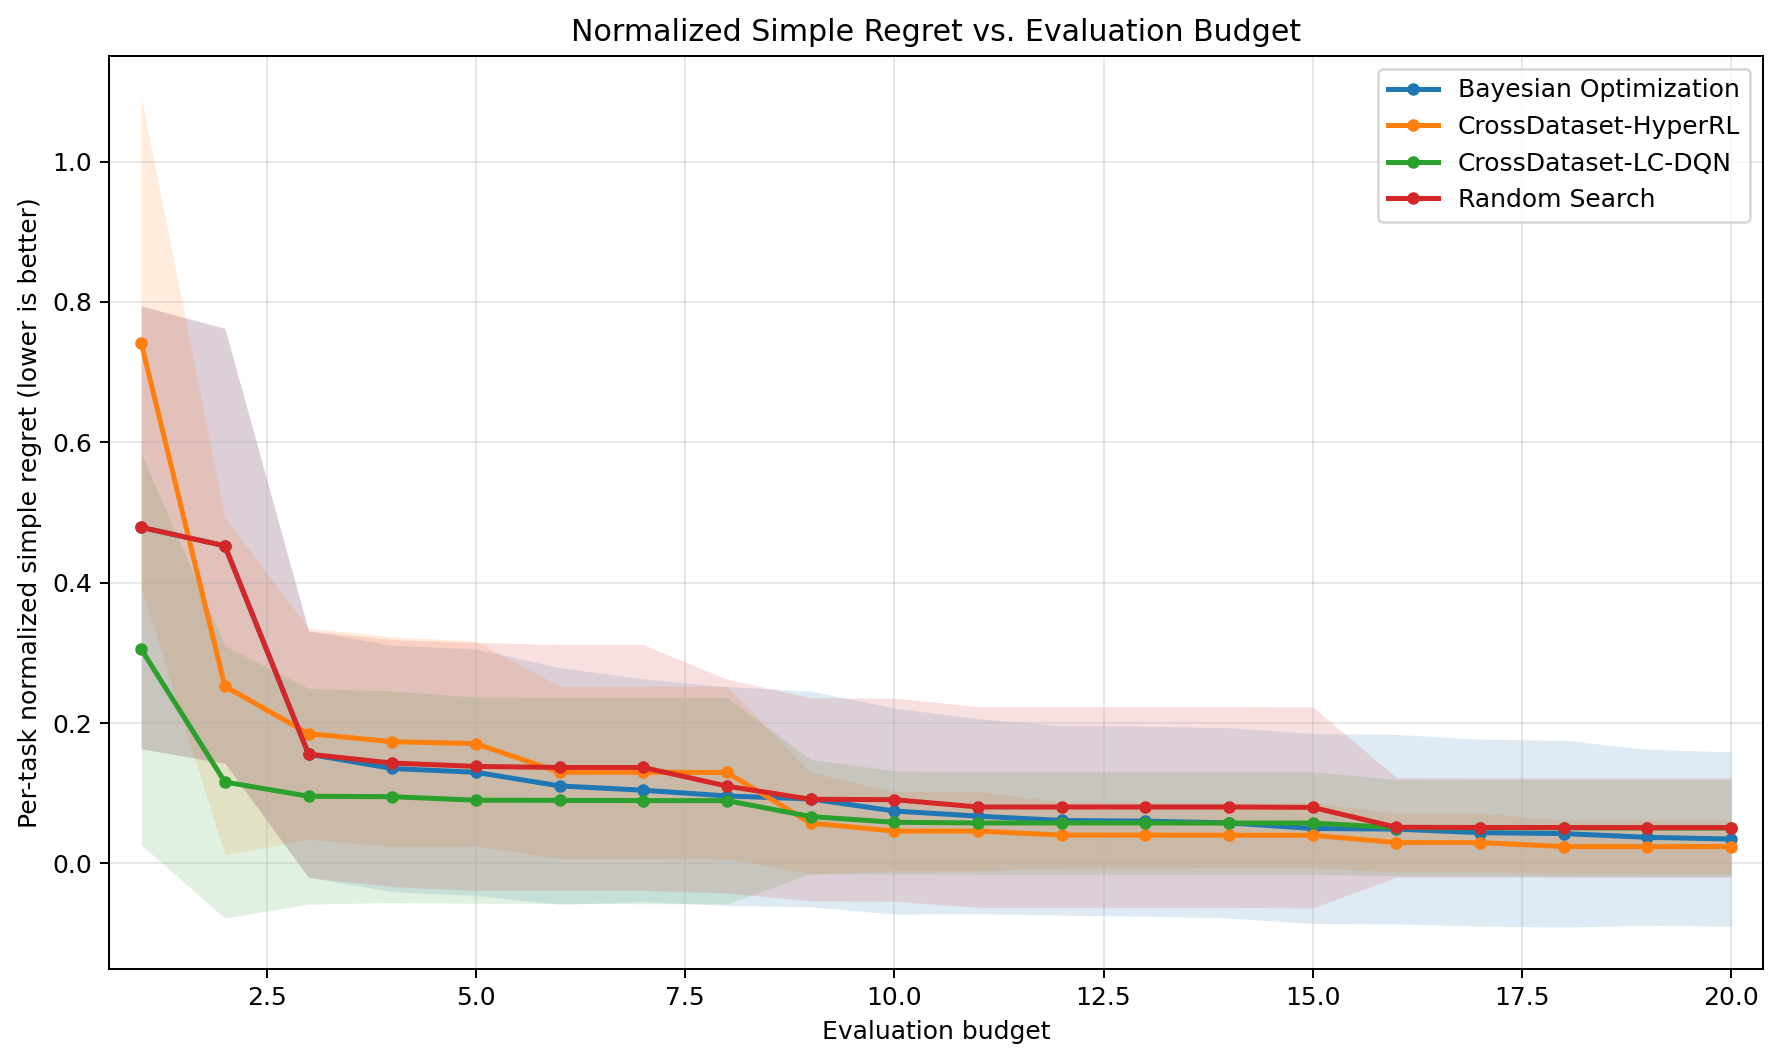
\includegraphics[width=\textwidth]{images/50_budget.png}
        \caption{Training Budget: 50}
        \label{fig:budget_50}
    \end{subfigure}
    
    % The empty line above and below the vspace is required to force a line break for the subfigures
    \vspace{0.5em}
    
    \begin{subfigure}[b]{0.48\textwidth}
        \centering
        % Insert the 100 budget image here
        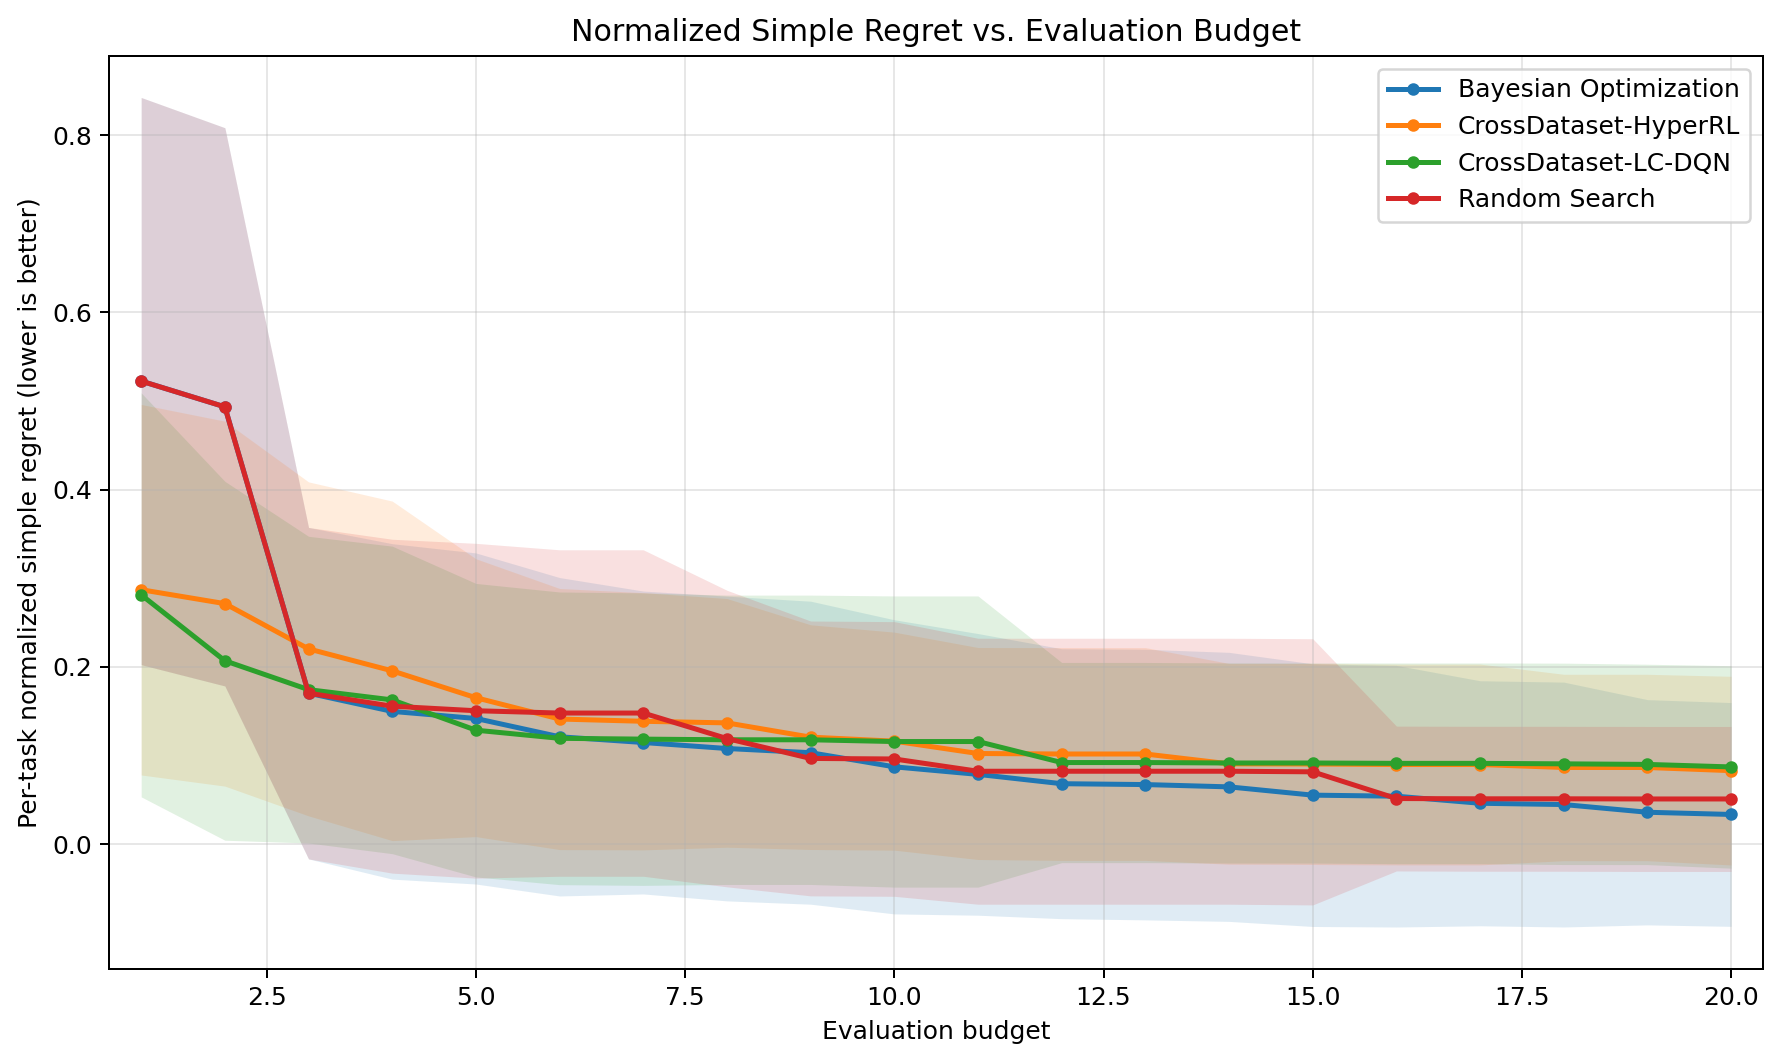
\includegraphics[width=\textwidth]{images/100_budget.png}
        \caption{Training Budget: 100}
        \label{fig:budget_100}
    \end{subfigure}
    \hfill
    \begin{subfigure}[b]{0.48\textwidth}
        \centering
        % Insert the 150 budget image here
        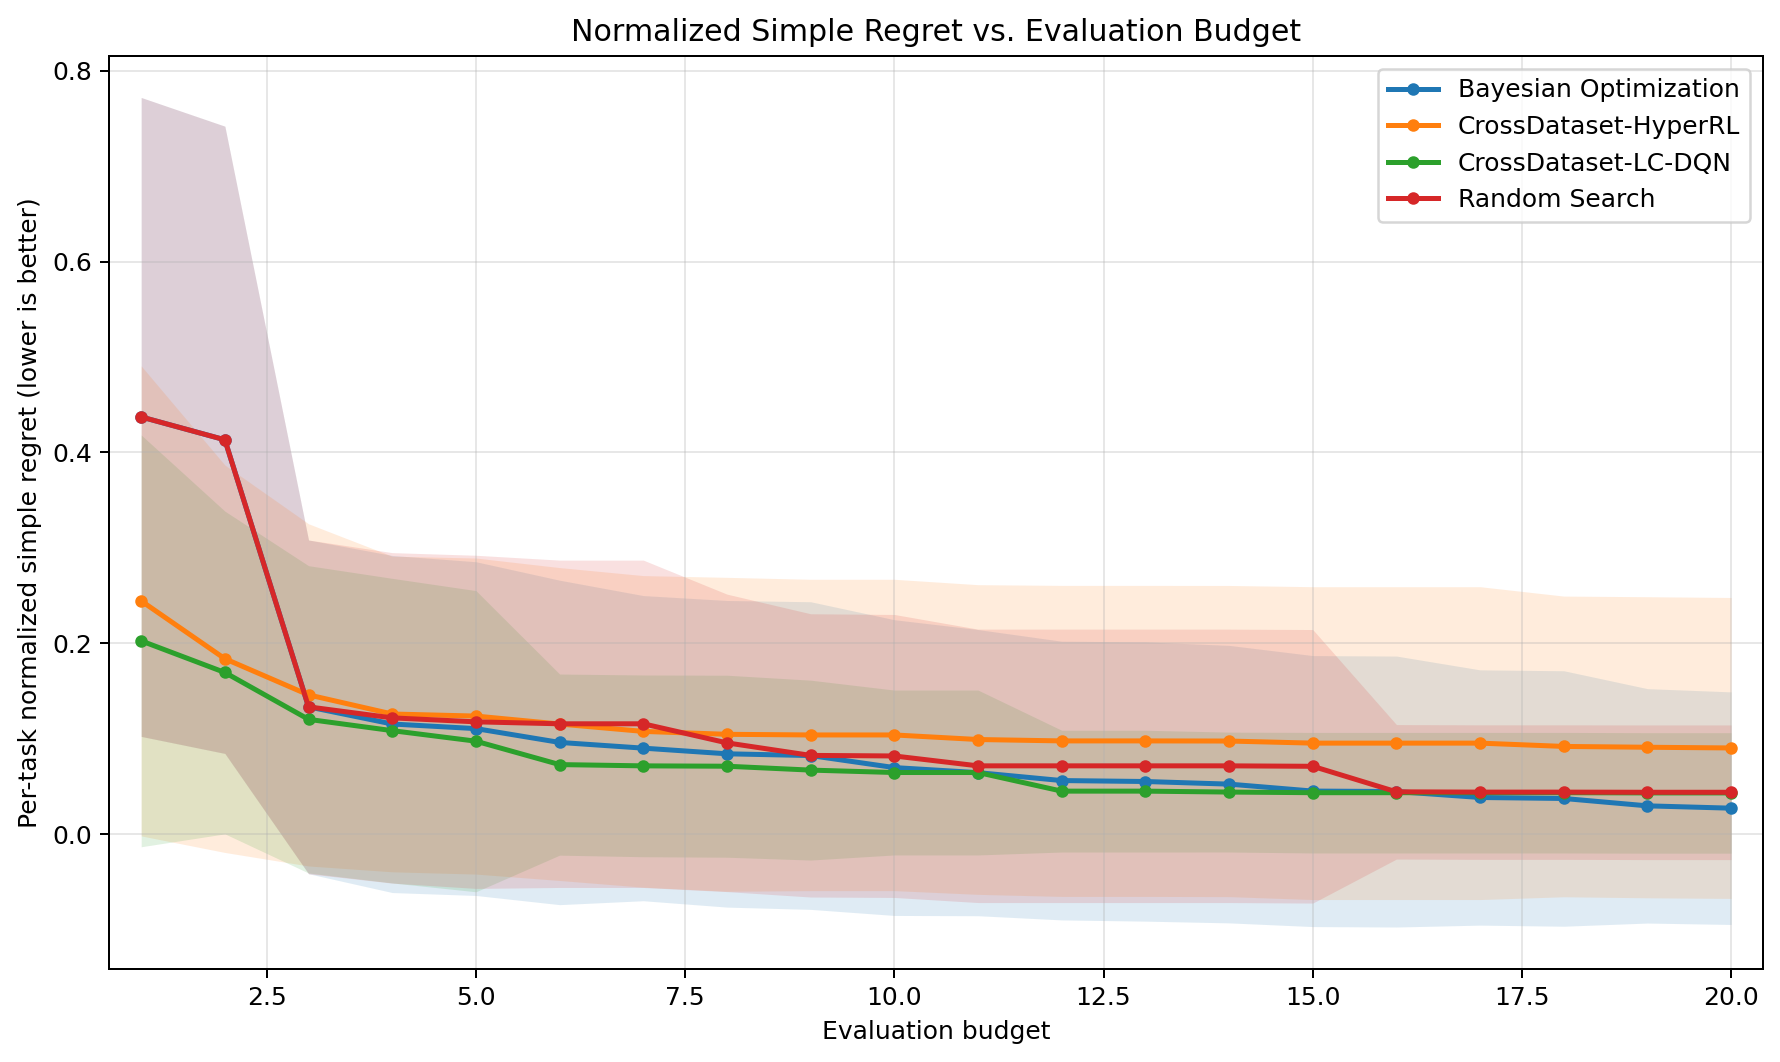
\includegraphics[width=\textwidth]{images/150_budget.png}
        \caption{Training Budget: 150}
        \label{fig:budget_150}
    \end{subfigure}
    \caption{Performance comparison of hyperparameter optimization methods across different training budget constraints. Lower validation scores indicate better performance.}
    \label{fig:hpo_results}
\end{figure}

\begin{itemize}
    \item \textbf{Initial Optimization Phase (Cold-Start):} At low evaluation budgets (e.g., trials 1 through 5), the \texttt{CrossDataset-HyperRL} and \texttt{CrossDataset-LC-DQN} methods yield lower validation scores compared to Bayesian Optimization and Random Search. This indicates a higher search efficiency and a more effective initialization during the early phase of the optimization process.
    \item \textbf{Meta-Learning and Knowledge Transfer:} This early-stage performance difference correlates with the underlying initialization mechanisms. \texttt{CrossDataset-HyperRL} utilizes metadata to transfer learned hyperparameter distributions from prior datasets to the current validation dataset. Conversely, standard Bayesian Optimization initiates the search process on each new dataset without prior external data, requiring more exploratory trials to model the objective function from scratch.
    \item \textbf{Asymptotic Convergence:} As the evaluation budget increases (beyond 15 to 20 trials), the validation scores of all evaluated methods converge to a similar numerical range. The data shows that given a sufficient evaluation budget, the surrogate model constructed by Bayesian Optimization achieves an equivalent performance level to the transferred policies of the meta-learning approaches.
\end{itemize}

\subsection{Cross-Dataset Transfer on the Kaggle Playground Series}
\label{section:exp:kaggle}

On LCBench, \texttt{CrossDataset-LC-DQN} and \texttt{CrossDataset-HyperRL} are essentially indistinguishable: at the smallest budgets the curve-free \texttt{HyperRL} ablation is even marginally ahead of the full method (e.g.\ the orange curve below the green one in Figure~\ref{fig:budget_20}). LCBench therefore cannot isolate the contribution of the derivative-informed state. To probe this, we meta-train the same two cross-dataset policies (\texttt{CrossDataset-LC-DQN} and \texttt{CrossDataset-HyperRL}) on the Kaggle source tasks and evaluate them with frozen weights on the 15 heterogeneous Kaggle Playground tasks, reporting per-task normalized simple regret against the evaluation budget (Figure~\ref{fig:kaggle_eval_budget}); normalization makes regret comparable across the widely varying loss scales of the suite.

\begin{figure}[htbp]
    \centering
    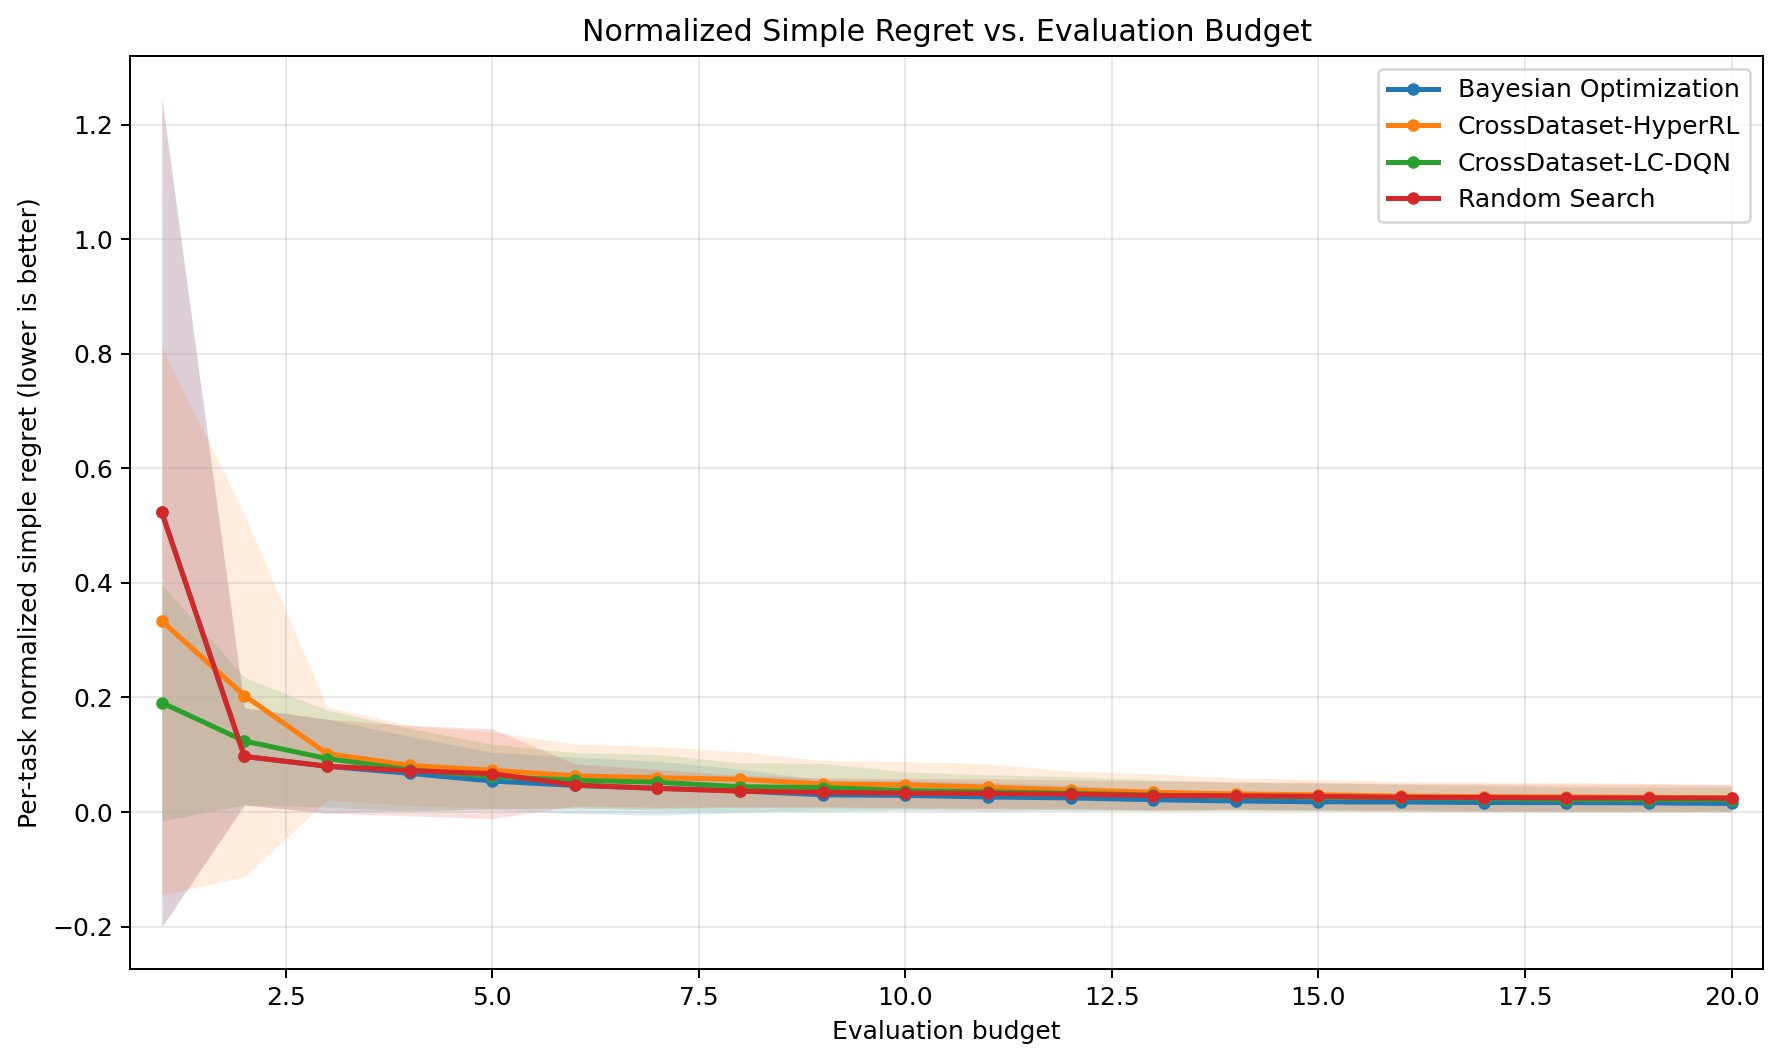
\includegraphics[width=0.72\textwidth]{images/kaggle_eval_budget.png}
    \caption{Normalized simple regret versus evaluation budget on the 15 Kaggle Playground tasks (5 seeds per task; shaded bands denote $\pm$ one standard deviation). Lower is better. Unlike LCBench, the curve-informed \texttt{CrossDataset-LC-DQN} (green) clearly separates from the curve-free \texttt{CrossDataset-HyperRL} (orange) throughout the cold-start region.}
    \label{fig:kaggle_eval_budget}
\end{figure}

\begin{itemize}
    \item \textbf{Derivative features isolate a measurable gain.} Across the low-budget region (trials 1--7), \texttt{CrossDataset-LC-DQN} sits consistently below \texttt{CrossDataset-HyperRL}. Averaged over all 15 tasks, its normalized simple regret is $0.0217$ versus $0.0251$ for \texttt{HyperRL}, and it also wins more tasks (rank-1 on 4 tasks vs.\ 2, average per-task rank $2.33$ vs.\ $2.87$). Because the two variants share the same policy, training protocol, and search space and differ \emph{only} in the appended learning-curve derivative statistics, this gap directly attributes the improvement to the derivative-informed state.
    \item \textbf{Curve features are what beat the random baseline.} The curve-free \texttt{HyperRL} ($0.0251$) is in fact slightly \emph{worse} than Random Search ($0.0243$) on average, whereas adding the derivative features pushes \texttt{LC-DQN} ($0.0217$) clearly below it. On this heterogeneous suite, cross-dataset policy transfer alone is not enough to outperform random sampling---the learning-curve signal is the deciding factor.
    \item \textbf{Bayesian Optimization remains strongest asymptotically.} As on LCBench, the GP surrogate attains the best overall normalized simple regret ($0.0150$) and dominates once the budget is large. The advantage of the transferred RL policies is concentrated in the early cold-start regime, where a learned prior matters more than an on-the-fly surrogate.
\end{itemize}

\paragraph{Why curve features help on Kaggle but not on LCBench.}
LCBench is deliberately homogeneous: every task trains the same funnel-shaped MLP family over the same 7-dimensional search space for a fixed 50 epochs, so the logged validation curves are smooth, stereotyped, and largely monotone. A configuration's final value is then well predicted by the static dataset descriptor and the scalar reward already present in the \texttt{HyperRL} state, leaving the derivative statistics (slope, curvature, recent improvement) with little additional signal---and at times adding input noise, which explains why \texttt{LC-DQN} fails to improve over \texttt{HyperRL} there. The Kaggle suite, by contrast, spans both regression and classification over real-world tabular datasets with very different scales and training dynamics, so different configurations produce genuinely diverse curve geometries (steady improvers, early plateaus, overfitters). In this setting the derivative features supply discriminative cold-start information that the scalar-only state lacks, letting the curve-informed policy commit to promising configurations sooner. In short, the derivative-informed state pays off precisely when learning-curve \emph{shape} varies across configurations---a property the heterogeneous Kaggle tasks exhibit and the uniform LCBench protocol largely removes.

\paragraph{Effect of meta-training task count.}
Figure~\ref{fig:kaggle_task_count} varies the number of source datasets used to meta-train \texttt{LC-DQN} ($1, 5, 10, 15$) and reports normalized simple regret on the held-out targets (75 runs per setting). Transfer does not improve monotonically with more source tasks: regret is lowest at 15 tasks ($0.0217$) but the curve is non-monotonic, peaking at 10. We read this as a consequence of the suite's heterogeneity---adding dissimilar source datasets injects conflicting reward scales and curve dynamics that a single shared LSTM must reconcile, so additional tasks help only once enough are present to average out the mismatch. The standard-error bars overlap substantially, however, so this trend is weak and should be treated as suggestive rather than conclusive.

\begin{figure}[htbp]
    \centering
    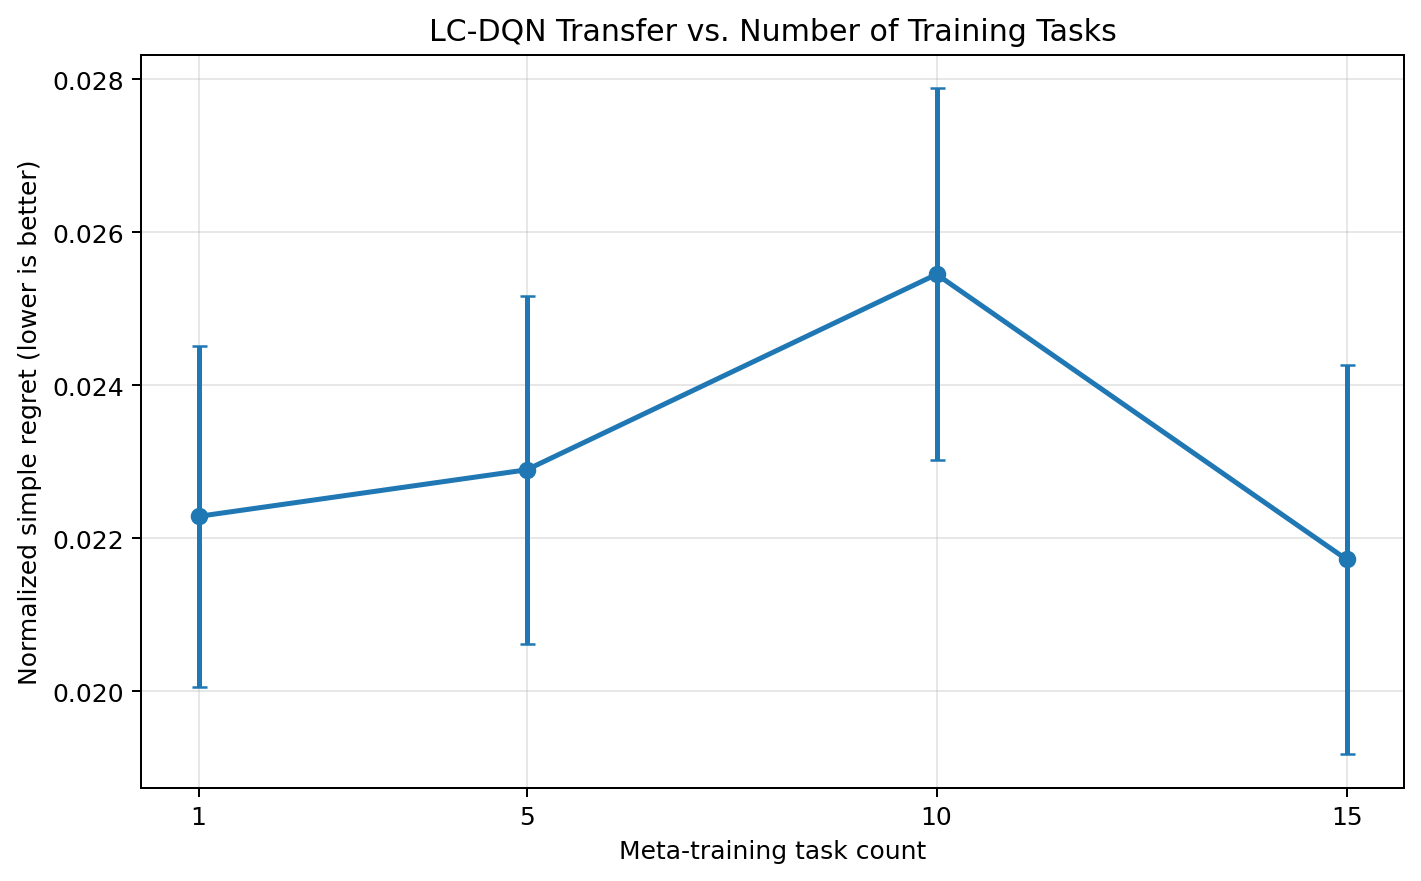
\includegraphics[width=0.6\textwidth]{images/kaggle_task_count.png}
    \caption{\texttt{CrossDataset-LC-DQN} transfer performance as a function of the number of meta-training (source) datasets. Error bars denote one standard error over 75 runs.}
    \label{fig:kaggle_task_count}
\end{figure}

